
\documentclass[a4paper,12pt]{article}
\usepackage[utf8]{inputenc}
\usepackage{graphicx}
\usepackage[spanish]{babel}
\usepackage{geometry}
\usepackage{caption}
\geometry{margin=2.5cm}

\title{Técnicas de Codificación - Segunda Señal}
\author{}
\date{}

\begin{document}

\maketitle

Este informe presenta seis técnicas comunes de codificación utilizadas en la transmisión digital de datos, aplicadas sobre una nueva secuencia binaria: \textbf{[0, 1, 1, 0, 1, 0, 0, 1]}.

\section*{1. Codificación NRZ (No Retorno a Cero)}

\begin{figure}[h!]
\centering
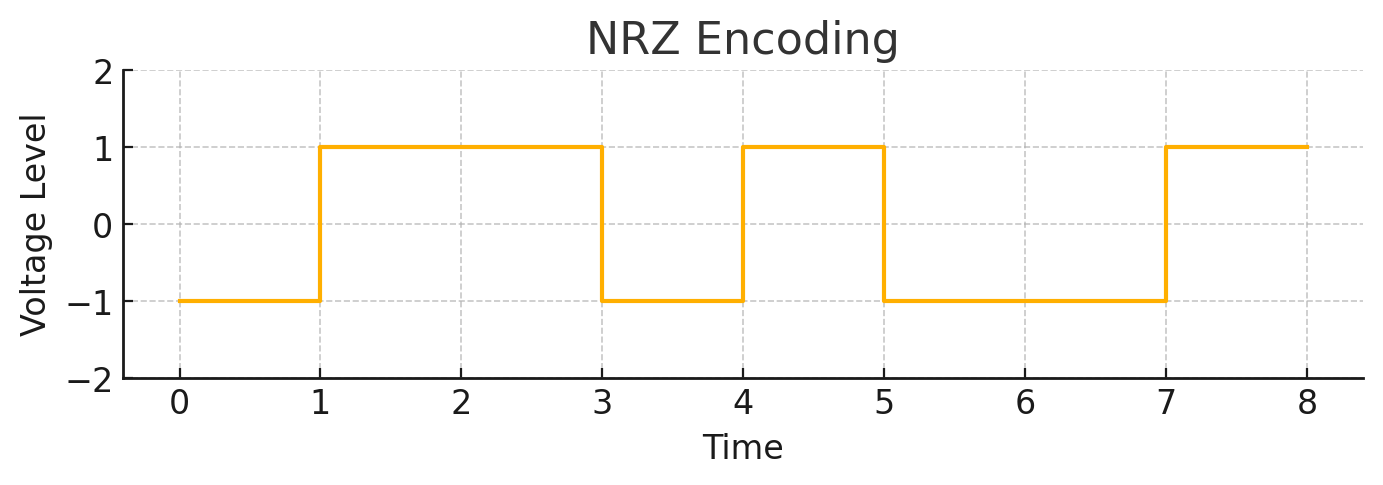
\includegraphics[width=0.9\textwidth]{nrz_v2.png}
\caption{Codificación NRZ}
\end{figure}

La técnica NRZ representa un '1' con un nivel de voltaje constante (positivo o negativo) y un '0' con el otro. No hay retorno a cero entre bits. Es simple pero puede generar problemas de sincronización con secuencias largas del mismo bit.

\clearpage

\section*{2. Codificación NRZI (No Retorno a Cero Invertido)}

\begin{figure}[h!]
\centering
\includegraphics[width=0.9\textwidth]{nrzi_v2.png}
\caption{Codificación NRZI}
\end{figure}

En NRZI, un bit '1' se representa por un cambio en el nivel de voltaje, y un bit '0' mantiene el mismo nivel. Esta técnica mejora la sincronización frente a NRZ en presencia de secuencias de '1'.

\clearpage

\section*{3. Codificación Manchester}

\begin{figure}[h!]
\centering
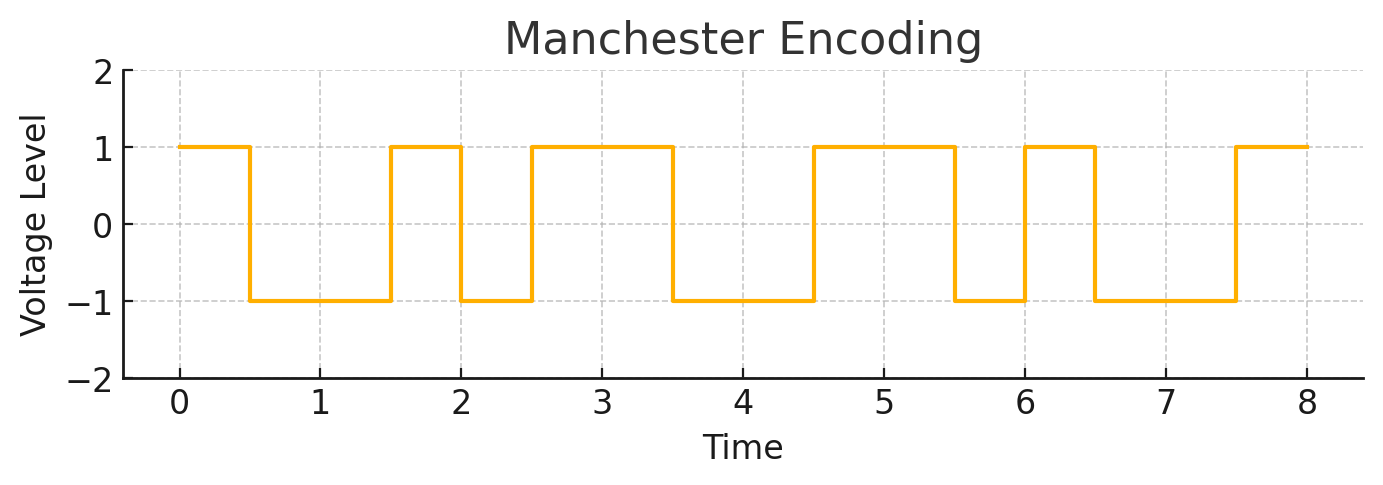
\includegraphics[width=0.9\textwidth]{manchester_v2.png}
\caption{Codificación Manchester}
\end{figure}

Cada bit tiene una transición en el centro del intervalo. Un '0' se representa por una transición de alto a bajo, y un '1' por una de bajo a alto. Garantiza sincronización al tener transiciones regulares.

\clearpage

\section*{4. Codificación Manchester Diferencial}

\begin{figure}[h!]
\centering
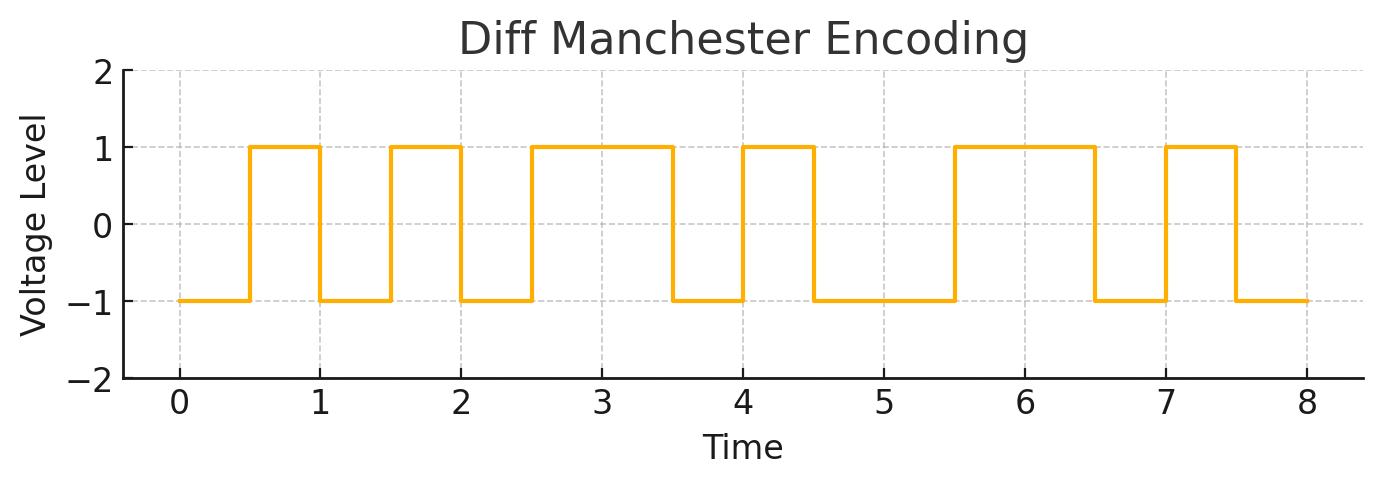
\includegraphics[width=0.9\textwidth]{diff_manchester_v2.png}
\caption{Codificación Manchester Diferencial}
\end{figure}

La codificación Manchester Diferencial se basa en una transición obligatoria en medio del intervalo de bit para mantener la sincronización. Un bit '0' cambia el nivel al inicio, un bit '1' lo mantiene. Es robusta frente a errores de sincronización.

\clearpage

\section*{5. Codificación Retorno a Cero (RZ)}

\begin{figure}[h!]
\centering
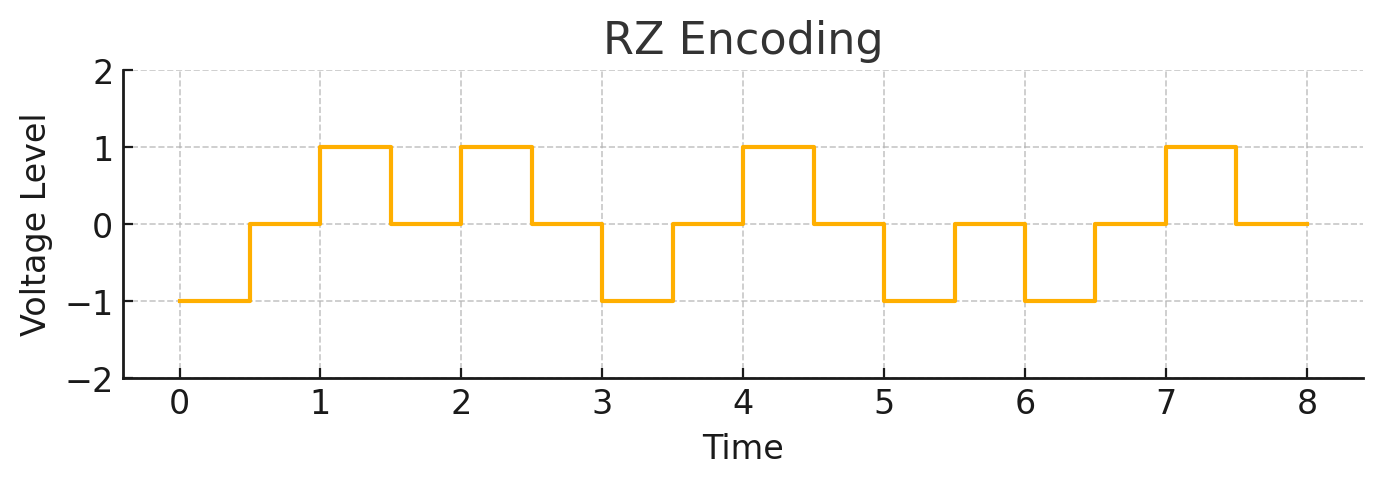
\includegraphics[width=0.9\textwidth]{rz_v2.png}
\caption{Codificación RZ (Retorno a Cero)}
\end{figure}

La técnica RZ utiliza tres niveles: positivo, negativo y cero. Cada bit tiene un pulso en la mitad inicial del intervalo y luego retorna a cero. Mejora la sincronización pero requiere mayor ancho de banda.

\clearpage

\section*{6. Codificación Bipolar (AMI)}

\begin{figure}[h!]
\centering
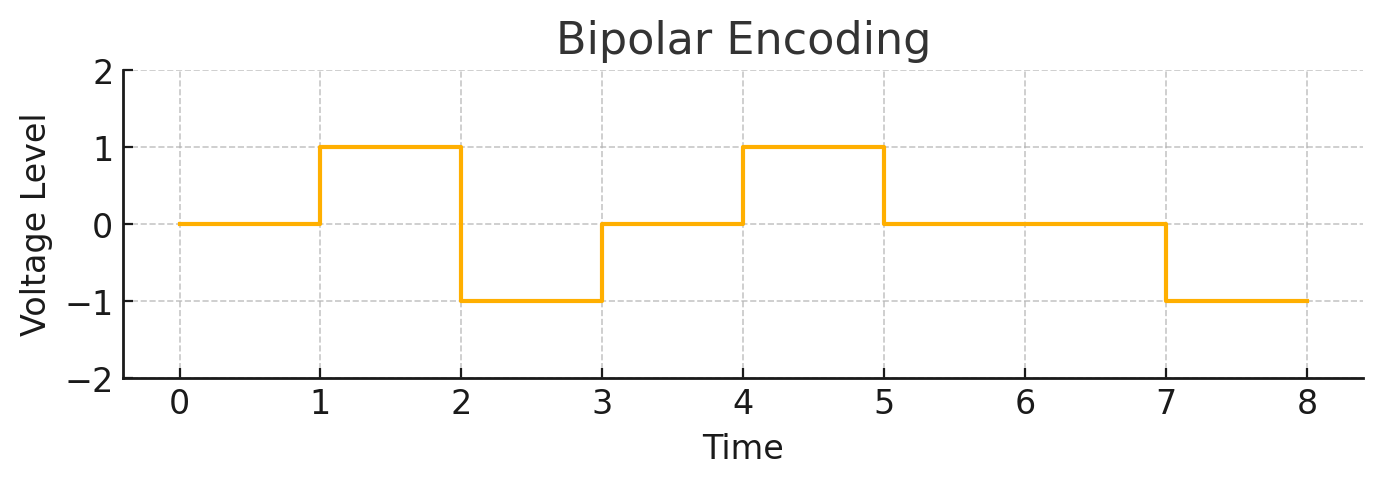
\includegraphics[width=0.9\textwidth]{bipolar_v2.png}
\caption{Codificación Bipolar (AMI)}
\end{figure}

La codificación Bipolar (AMI) representa los '0' con nivel cero, mientras que los '1' alternan entre niveles positivos y negativos. Esto facilita la sincronización y permite la detección de errores.

\end{document}
